%base packages 
\documentclass[11pt]{article}
\usepackage[margin=1in]{geometry}
\usepackage{caption,multirow,etoolbox,color,enumerate,amsmath,dsfont,lscape,tocloft,booktabs,draftwatermark,array,tabularx,graphicx,pdflscape,subcaption,comment}
\usepackage{setspace}
\setlength{\parskip}{0em}
\usepackage[bottom, flushmargin]{footmisc}
\usepackage[T1]{fontenc}
\usepackage[utf8]{inputenc}
\usepackage{lmodern}
\usepackage[english]{babel}
\usepackage[autostyle]{csquotes}
\makeatletter
\makeatother
\usepackage{float}
\SetWatermarkText{}\SetWatermarkLightness{0.85} \SetWatermarkScale{4}
\usepackage{appendix}
\usepackage{authblk}
\usepackage[format=hang,justification=raggedright,singlelinecheck=0,labelsep=period]{caption}
%[format=hang,justification=raggedright,singlelinecheck=0,labelsep=period]
%\usepackage[numbers,sort&compress]{natbib} %Use this set-up for numbered reference lists
\usepackage[authoryear]{natbib} %Use this set-up if you want an un-numbered reference list
%\usepackage{hypernat}

\usepackage[hyperfootnotes=false]{hyperref}
%\usepackage[dvipdfmx,hyperfootnotes=false]{hyperref}
%\usepackage[dvips,hyperfootnotes=false]{hyperref}
\hypersetup{colorlinks=true,linkcolor=blue,anchorcolor=blue,citecolor=blue,filecolor=blue,urlcolor=blue,bookmarksnumbered=true,pdfview=FitB} %
% % %DO NOT PLACE ANY PACKAGES AFTER THE HYPERREF SET UP
\usepackage{titling}

%-----------------------------------------------------------------------%
\begin{document}
\bibliographystyle{apa-good}


\title{Side-Selling and the Impact of Participating in Smallholder Livestock Cooperatives in Nepal\thanks{Copyright 2020 by Scott M. Miller (\href{scottmmiller@ufl.edu}{scottmmiller@ufl.edu}). All rights reserved. Readers may make verbatim copies of this document for non-commercial purposes by any means, provided this copyright notice appears on all such copies.} \thanks{This work was funded in whole or part by the United States Agency for International Development (USAID) Bureau for Food Security under Agreement # AID-OAA-L-15-00003 as part of Feed the Future Innovation Lab for Livestock Systems. Any opinions, findings, conclusions, or recommendations expressed here are those of the authors alone.}}

\author{Scott M. Miller}
\date{}

\sloppy
\maketitle



\vspace{2cm}
%------------------------------------------%
%\begin{abstract}
%Agricultural cooperatives have long been viewed as an important tool for promoting agricultural development and alleviating poverty around the world. Despite this potential, the success of many cooperatives is limited by their inability to successfully coordinate sales and reduce market constraints. This failure is apparent in livestock cooperatives across rural Nepal, where over 80\% of cooperative members engage in side-selling despite evidence that those who sell through the cooperative receive a higher price and sell more goats on average. In order to estimate the average impact of cooperative goat sales, I combine model selection via the LASSO with doubly robust treatment effect estimation. 
%\end{abstract}
%------------------------------------------%

\pagenumbering{gobble}

\clearpage
\doublespacing
\thispagestyle{plain}
\pagenumbering{arabic}
\setcounter{page}{1}

%-----------------------------------------------------------------------%
\section{Introduction} \label{sec:intro}
% Hook
Agricultural cooperatives are widely viewed as an important tool for increasing the production and commercialization of smallholder producers in developing countries \citep{poole_review_2010}. Despite evidence that cooperative membership can increase the productivity and incomes of smallholders in certain settings \citep{bernard_impact_2008,fischer_linking_2012,ma_does_2016}, many cooperatives struggle to maintain market competitiveness. Cooperatives often experience a high presence of side-selling, heterogeneous benefits, or dissolving participation among their members \citep{aflagah_cheap_2019,bernard_reaching_2009,casaburi_loyalty_2015}. 

One of the most important failures of agricultural cooperatives takes the form of side-selling, in which cooperative members choose to sell their output to a local trader, often subverting the best interest of the organization and its members. Side-selling is detrimental to marketing cooperatives, whose ability to benefit smallholders partially depends on the market power generated from pooling a large quantity of its members' output and collectively bargaining for good prices. Yet this phenomenon is widespread in livestock cooperatives across rural Nepal, where over 80\% of goat-selling households choose to sell their goats to a local trader instead of through the cooperative of which they are a member. What makes this problem more interesting is evidence that those who sell through their cooperative receive a higher price and sell more goats on average than do the side-selling households. 

% question
Are cooperative sales more beneficial for smallholders than outside sales in this setting? And if so, why do so few producers sell through the cooperative of which they are a member? In order to answer these questions, I use a two-way fixed effects model to estimate the impact of selling goats through the cooperative as opposed to side-selling. I then explore treatment effect heterogeneity to investigate why a small number of producers sell through the cooperative, shedding light on the distributional returns to cooperative participation. 

My population of interest consists of smallholder goat producers in rural Nepal, all of whom are women and members of agricultural cooperatives. All cooperatives included in this study were organized by Heifer Project International Nepal (HPIN), an NGO that provides a number of services to smallholders in rural Nepal. The data used in this study cover 2,856 households across 108 cooperatives. This data set consists of two separate surveys --- one with cooperative leaders and another with general members. The separate questionnaires for cooperative members and leaders provides a number of benefits for this study. The cooperative leader survey provides institutional information about each cooperative and its overall performance. The household survey collects detailed information on a sample of members from each cooperative, including their individual performance as a producer. The ability to link member-level data to each cooperative's organizational structure provides the unique ability to account for both individual and institutional factors when estimating the ATT. % re-write this section (taken from previous paper)

% Antecedents
While a number of empirical studies have analyzed side-selling in the case of agricultural cooperatives in developing countries, most consist of case studies of a small number of organizations. \citet{shumeta_two-step_2018} analyze the determinants of side-selling among 12 coffee cooperatives in Ethiopia and find that age, education, off-farm income and trust in cooperative leadership decrease side-selling, while larger group size and delayed payments increase side-selling in this context. \citet{getnet_power_2018} analyze a small sample of sesame producers in Ethiopia and suggest that cooperatives sales are associated with higher prices and incomes for the participating smallholders.  \citet{wollni_member_2015} develop a theoretical model of cooperative side-selling and test this model with a sample of four coffee cooperatives in Costa Rica. The theoretical and empirical results demonstrate a U-shaped relationship between farm size and side-selling. \citet{mujawamariya_exploring_2013} use the case of four coffee cooperatives in Rwanda to investigate double side-selling, in which some cooperative members sell their output to local traders and a number of non-members sell to cooperatives. The authors find that the additional transaction costs associated with cooperative sales, in addition to late payments, are an important determinant of side-selling that is often overlooked in a standard cost-benefit analysis.

The main exception in the cooperative literature to small case studies of side-selling is the paper by \citet{aflagah_cheap_2019}, who combine a lab-in-the-field experiment with a randomized control trial to analyze the effect of cheap talk (revealing farmers' intentions to sell through or outside of their cooperative) on collective commercialization. Studying nearly 900 farmers across 79 groundnut-producing cooperatives in Senegal, \citet{aflagah_cheap_2019} find that revealing farmers' intended cooperative sales improved collective commercialization, particularly in larger groups, and that this intervention may lead to higher incomes for small-scale farmers. 

% Value Added
This paper builds on the cooperative literature by using a large data set to analyze the impact of cooperative participation. By studying more than 2,500 members across 108 cooperatives, this paper provides a significantly larger sample size than most prior studies, allowing for a more rigorous analysis of member selling decisions and a detailed exploration of treatment effect heterogeneity. Additionally, prior studies on this topic have largely analyzed the case of seasonal crop production. This paper focuses on smallholder livestock production, a commodity that has rarely been studied in the cooperative literature. Livestock producers face a considerably different set of choices and constraints than seasonal crop producers. In particular, livestock need not be harvested and sold at any specific point in time, but provide producers with the ability to optimize their sales timing --- taking into account animal weight, market conditions, and household financial needs.

% Results
I find that selling goats through the cooperative leads to an 18\% increase in price compared to outside sales, on average. I find no significant impact on the number of goats sold. 
 


%-----------------------------------------------------------------------%
\section{Conceptual Framework} \label{sec:background}

Smallholder producers in developing countries often face constraints that limit their ability to sell in formal markets \citep{barrett_smallholder_2008}. These constraints include poor infrastructure, weak communication channels and long distances between market actors that lead to high transaction costs, weak bargaining power and information asymmetry \citep{aker_information_2010,key_transactions_2000,staal_smallholder_1997}. Agricultural cooperatives may contribute to productivity growth and poverty alleviation by helping smallholders increase bargaining power, decrease transaction costs, and achieve scale economies in marketing \citep{markelova_collective_2010,staal_smallholder_1997,csaki_reaching_2003}. 

Through collective action, cooperatives provide the opportunity for smallholders to access markets that may otherwise be inaccessible, pool resources to overcome financial constraints, increase communication flows and collectively negotiate with buyers to receive better prices \citep{poole_review_2010}. But rather than eliminating the source of market constraints, the burdens are shifted to the cooperatives themselves. The effectiveness of cooperatives in raising smallholder market engagement often depends on how well cooperatives manage the challenge of internally coordinating sales among a large group of individual market actors.

Cooperatives frequently fail to overcome this challenge, facing problems such as free-riding and side-selling that damage market performance and disincentivize further participation. Smallholders stand to benefit from joining a cooperative in order to access a number of services \citep{fischer_smallholder_2014} such as subsidized inputs, market information, veterinary support and loans. But in order for collective action to improve market conditions, a critical mass of participation in activities like group marketing is required \citep{aflagah_cheap_2019}. In cases where active participation is not enforced and the marginal cost of participation is high, there may be an incentive to reap the benefits of membership without adequately contributing to the organization's success \citep{fischer_smallholder_2014}.

Side-selling is particularly damaging to marketing cooperatives, who pool their members' output in an attempt to bargain for better prices. When members subvert the cooperative and sell directly to the market, they undercut the cooperative's negotiations and potentially lower the price for participating members. This weakens the incentive to participate in future sales, which may serve to further decrease the cooperative's bargaining power. 

Members may choose to side-sell for a number of reasons, including the delayed payment structure employed by many cooperatives \citep{markelova_collective_2010,mujawamariya_exploring_2013,shumeta_two-step_2018}. Additionally, the price received for cooperative sales does not always outweigh the full set of costs incurred in cooperative participation, including transaction costs. \citet{aflagah_cheap_2019} argue that the price received through collective commercialization is dependent on the cooperative reaching a critical mass of participation in a given sale. Under this framework, cooperatives are able to offer a higher price than local traders if they are able to aggregate sufficient production and successfully negotiate for better contracts \citep{aflagah_cheap_2019}. But if cooperatives fail to aggregate a sufficient quantity or successfully negotiate, farmers may have to resort back to side-selling. In this scenario, the combination of long waiting times and high transaction costs may lead to a lower effective price than would have been received at farmgate \citep{aflagah_cheap_2019}.


\subsection{Livestock Cooperatives in Nepal}

In Nepal, where 68 percent of the population depends on agriculture for their livelihood \citep{international_labor_organization_ilo_2016}, goats are a common source of income and nutrition. This is particularly true in rural areas, where nearly every household owns a least a few goats for production and/or consumption \citep{upreti_food_2009}. The majority of goats in Nepal are consumed after sale to a local collector who pools animals from smallholder producers \citep{heifer_international_nepal_study_2012}. For goats that are marketed outside of their original communities, the commercial value chain links producers, local collectors and regional traders to consumers who are primarily located in urban markets \citep{heifer_international_nepal_study_2012}. %A collector looking to buy goats from smallholder producers who are not affiliated with a cooperative would likely have to conduct individual negotiations, sometimes making multiple visits per home \citep{heifer_international_nepal_study_2012, staal_smallholder_1997}. After agreeing to terms with producers, the collector would still have to coordinate transportation. If the collector does not want to transport goats from each individual home, then he or she would have to arrange for producers to bring their animals to a collection point at a specific date and time. Bargaining with many small producers and managing logistics may inflate transaction costs and dissuade collectors from dealing with smallholders. In contrast, a collector purchasing through a cooperative need only negotiate with a single entity and can leave sales coordination to cooperative managers.

In the current setting, there are a number of additional considerations that may affect farmers' selling decisions. While there is a national festival season in which the demand for goat meat spikes over the course of several months (see section \ref{sec:sidesell}), goat production and sales do not follow the standard seasonal structure of crop production. Although the majority of farmers time their goat production for sale during the festival season (see figure \ref{figure:E2_month}), farmers may face liquidity constraints or shocks that force them sell at inopportune times. Cooperative sales during the festival season are likely to provide farmers with high prices, but the availability of year-round sales provides them with the opportunity to side-sell at a lower price to quickly receive funds if needed. 

The combination of Nepal's mountainous landscape and poor infrastructure may also affect the transaction costs incurred in cooperative sales. Participating in collective commercialization in this context often requires farmers to directly transport their goats to the cooperative's collection center, which may be several miles away and involve significant changes in altitude. If the farmer does not have access to some form of large-scale transportation (such as a truck to carry their goats), farmers will need to walk their herd to the cooperative's location. On the other hand, many local traders directly visit producers' homes and offer to transport their goats if a sale is finalized. While the trader is likely to offer a lower price, the time and effort saved in transportation may offset this difference.

% communication and inclusion (awareness of sales)
Cooperatives in this setting appear to struggle with coordinating goat sales in a way that is inclusive of members \citep{mullally_impact_2020}. Although officers from 86\% of cooperatives in the sample stated that their organizations coordinated goat sales, only 35\% of households received information about a cooperative sale in the six-months prior to data collection. These cooperatives also appear to largely communicate in person. Less than 30\% of households in our sample received any information about sales organized through the cooperative in the 6 months prior to data collection. Among the households that did receive price and sales information, nearly 75\% did so through in-person meetings. Distance to meeting points could be a barrier to more frequent interactions, as cooperative members state that it takes approximately 90 minutes to travel to and from cooperative meetings, on average. Cooperatives may be responding slowly to market demand and potentially losing sales in the time it takes to communicate with members, while also failing to consider the entire inventory of animals at their disposal.

%-----------------------------------------------------------------------%
\section{Data} \label{sec:data}
In this paper I use a cross-sectional dataset covering 2,856 households across 108 female smallholder livestock cooperatives in Nepal. The cooperatives in this sample are spread across four of five development regions in Nepal, specifically the East, Central, West and Mid-Western Development regions. All cooperatives operate in either the low-land Terai or mid-Hills. Figure (\ref{map}) shows the study area covered in the sample, which includes cooperatives from 24 districts across Nepal. The cooperatives included in the study were selected by HPIN and include all existing livestock marketing cooperatives the organization helped form prior to 2017.

This dataset consists of two separate surveys - one with cooperative leaders and another with general members.
I refer to these surveys as the cooperative leader and household survey, respectively. The cooperative leader survey is comprised of interviews from three officers in each cooperative. To obtain a representative sample for the household survey, HPIN and cooperative leaders generated complete cooperative rosters. From these comprehensive lists, a random sample of members from each cooperative was drawn to participate in the household survey. The data were collected from the sample in January 2018 using Android tablets and Open Data Kit.

\begin{figure}[!h]
    \caption{Study Area}
    \label{map}
    \noindent \centering 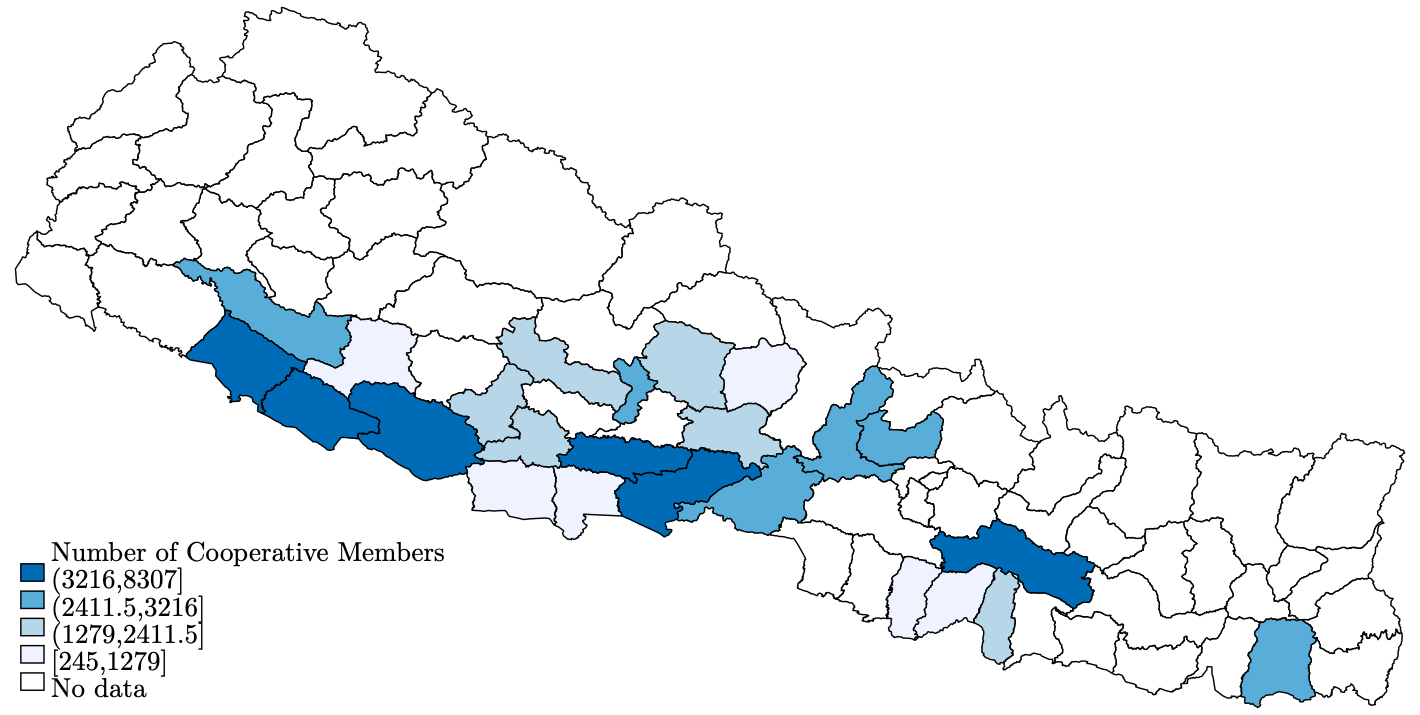
\includegraphics[width=.9\textwidth,trim=4 4 4 4,clip]{StudyMap.png}
\end{figure}

Table (\ref{table:summary}) displays summary statistics from the 2018 sample of my data. The average cooperative in my sample has 569 members, and a revenue of over \$3,800 USD. On average, cooperatives operate with a net revenue of roughly \$3,300 USD. However, there is significant heterogeneity in this measure, as average net revenue ranges from below -\$16,600 to more than \$65,500 USD. The average cooperative owns fewer than one information and communication technology (ICT) asset, but owns nearly 3 non-ICT assets. The average cooperative member in my sample is 42 years old, roughly 80\% of whom are literate. While the average household owns more than 5 goats, only 48\% sold a goat in the year prior to data collection and only 35\% received sale information from their cooperative in the 6-months prior to data collection. This may in part explain the disparity between goat sales through and outside of the cooperative. On average, goat-selling households sold more than two goats and received a revenue of \$85.07 USD per goat. Meanwhile, among goat-selling households the average number of cooperative goats sold is 0.53 and the average revenue per cooperative goat sold is \$91.44.

%\newpage
\singlespacing
% Summary Stats Table
\newcolumntype{Y}{>{\centering\arraybackslash}X}
\begin{table}[H]
  \centering
  \caption{Summary Statistics}
  \label{table:summary}
  \scalebox{.8}{
  \begin{tabularx}{1.2\linewidth}{l*{7}{Y}}
\hline Cooperative-Level Variables & N & Mean & sd & Min & Max\\
\noalign{\smallskip}\hline \noalign{\smallskip}
Number of Members (count) & 107.00 & 568.64 & 375.77 & 11.00 & 2,600.00\\
Annual Revenue (USD) & 108.00 & 3,862.05 & 7,503.18 & 0.00 & 65,709.51\\
Annual Costs (USD) & 108.00 & 624.62 & 2,619.28 & 0.00 & 21,383.74\\
Annual Net revenue (USD) & 106.00 & 3,298.52 & 7,929.31 & -16,676.6 & 65,554.2\\
Annual Revenue per member (USD) & 108.00 & 7.26 & 10.34 & 0.00 & 63.53\\
Annual Net revenue per member (USD) & 105.00 & 6.44 & 10.94 & -29.78 & 63.53\\
Annual Goat revenue (USD) & 106.00 & 173.05 & 542.82 & 0.00 & 5,262.24\\
Planning time horizon (years) & 108.00 & 1.33 & 1.07 & 0.00 & 5.00\\
ICT assets (count) & 108.00 & 0.62 & 0.71 & 0.00 & 3.00\\
Non-ICT assets (count) \hspace{2.15in} & 108.00 & 2.85 & 2.36 & 0.00 & 15.00\\


  \end{tabularx}}
  \scalebox{.8}{
  \begin{tabularx}{1.2\linewidth}{l*{7}{Y}}
\hline Household-Level Variables & N & Mean & sd & Min & Max\\
\noalign{\smallskip}\hline \noalign{\smallskip}
Age of female cooperative member (years) & 2,856.00 & 42.35 & 11.58 & 20.00 & 83.00\\
Literacy of female cooperative member (0/1) & 2,856.00 & 0.79 & 0.36 & 0.00 & 1.00\\
Contacted about cooperative sales in last 6-months (0/1) & 2,856.00 & 0.35 & 0.48 & 0.00 & 1.00\\
Total number of goats owned (count) & 2,856.00 & 5.76 & 4.95 & 0.00 & 69.00\\
Household sold goats in the last 12-months (0/1) & 2,856.00 & 0.48 & 0.50 & 0.00 & 1.00\\
Household side-sold goats in the last 12-months (0/1) & 1,384.00 & 0.77 & 0.42 & 0.00 & 1.00\\
Annual number of goats sold (count) & 1,384.00 & 2.31 & 1.85 & 1.00 & 10.00\\
Annual number of cooperative goats sold (count) & 1,384.00 & 0.53 & 1.05 & 0.00 & 4.00\\
Annual revenue per goat (USD) & 1,384.00 & 85.07 & 37.15 & 0.00 & 178.20\\
Annual revenue per cooperative goat (USD) & 353.00 & 91.44 & 30.08 & 0.00 & 135.13\\
Annual net goat income (USD) & 1,384.00 & 148.41 & 159.81 & -284.13 & 725.67\\
\hline
\multicolumn{6}{@{}p{1.2\textwidth}}
{\textit{Notes}: At the household-level, several variables include missing values and are conditional the household selling goats. These variables include: household side-sells goats, total goats sold, cooperative goats sold, revenue per goat and net goat income. Revenue per cooperative goat sold is conditional on the household selling goats through the cooperative.}
  \end{tabularx}}
\end{table}
\doublespacing

This dataset includes a module on each producer's goat sales, collecting detailed information on every sale that was made in the year prior to data collection. This information includes the sales channel (cooperative, local trader, relative, etc.), the number of goats sold, revenue, the size and type of goat sold as well as a number of other considerations. When analyzing the impact of cooperative sales, I use the data at the sale-level, rather than aggregating all sales across each producer. This allows me to individually analyze the decision to side-sell for each individual sale made. 


\subsection{Side-Selling} \label{sec:sidesell}

In this section, I describe the extent to which producers side-sell in my data. Figure (\ref{figure:E2_month}) displays the total number of goats sold through and outside of the cooperative by month in the year prior to data collection.\footnote{The calendar year in Nepal begins in mid-April.} This figure shows the extensive presence of side-selling throughout the year, with the number of goats sold outside of the cooperative often more than double the number sold through the cooperative. The highest presence of side-selling occurs during the Nepali festival season (August-December), where there is a spike in the demand for goat meat surrounding holiday celebrations.\footnote{Goat meat is significantly more expensive than many alternatives and is considered a luxury product in Nepal.} This figure indicates that cooperatives are failing to capture the majority of goat sales happening among their membership. 

\vspace{.5cm}
\begin{figure}[H]
    \caption{Total Number of Goats Sold by Sale Channel and Month}
    \label{figure:E2_month}
    \noindent \centering 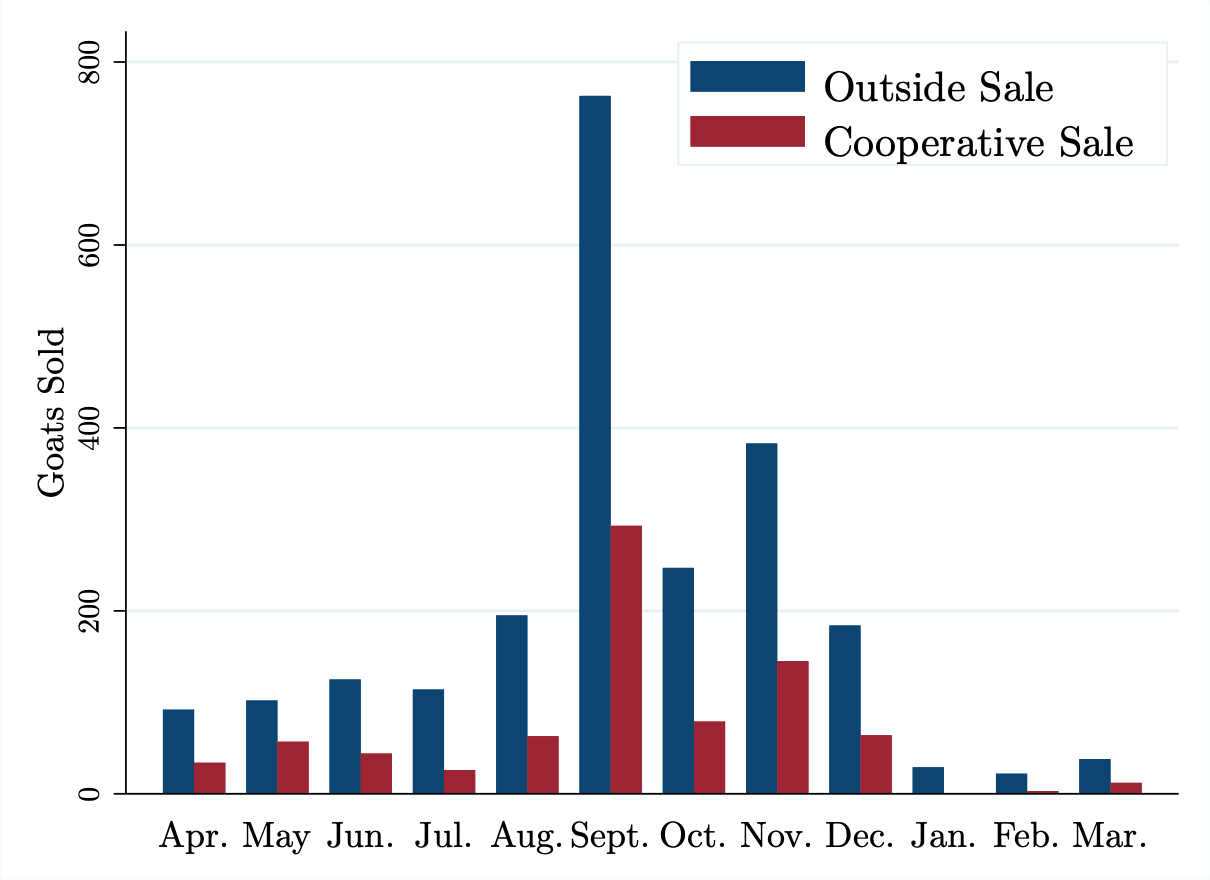
\includegraphics[width=.45\textwidth,trim=4 4 4 4,clip]{E2_SaleMonth.png}
\end{figure}

Figures (\ref{figure:E2_PD_Annual}-\ref{figure:E2_PD_NonFest}) display the distribution of goat prices received through each sale channel for the full calendar year, during festival season and outside of festival season. These figures suggests that selling goats through the cooperative may be more lucrative than side-selling, regardless of the timing of the sale. While the distribution of observed prices may suggest that cooperative sales are more beneficial, it is not clear whether each potential sale follows this pattern. Given the additional transaction costs associated with cooperative sales, it is possible that producers only choose to sell through the cooperative when the price is significantly higher than what is being offered by local traders. In this scenario, we would not expect to see cooperative sales occur when the price is less than or equal to the price of outside sales, potentially distorting what we can learn from observed sales. Solving this empirical puzzle requires identifying the impact of cooperative sales compared to similar outside sales.

\begin{figure}[H]
\caption{Distribution of Goat Prices by Sale Channel}
    \centering
    \begin{subfigure}[t]{.4\textwidth}
    \centering
        \caption{Annual} \label{figure:E2_PD_Annual}
        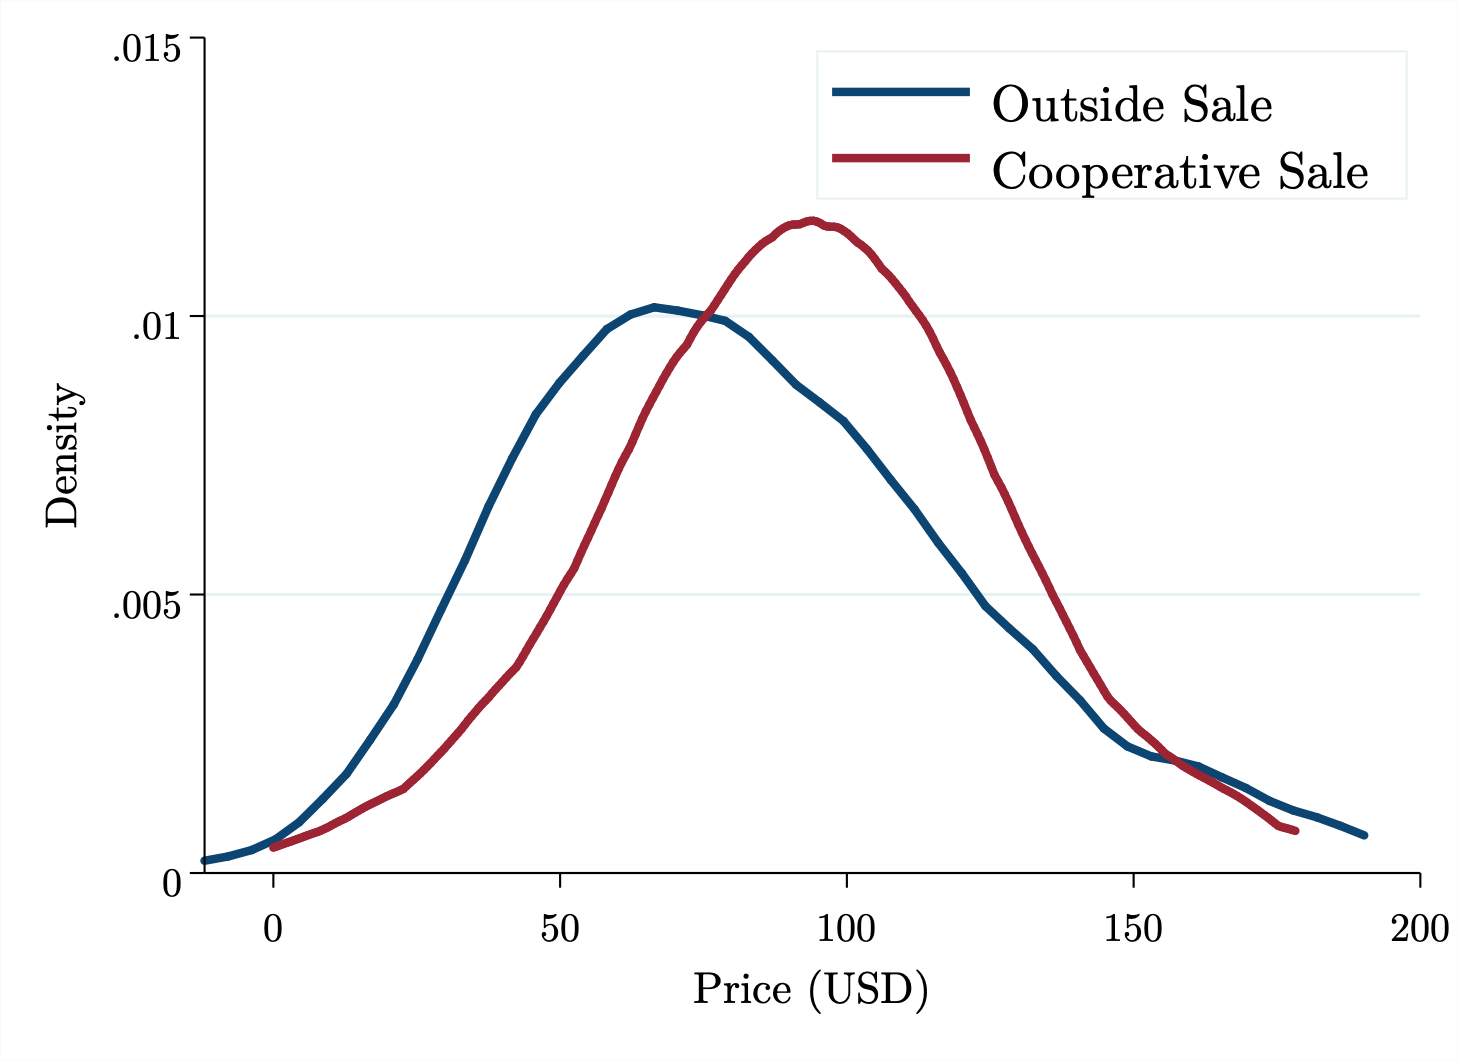
\includegraphics[width=\linewidth,trim=4 4 4 4,clip]{E2_PriceDensity_Annual.png} 
    \end{subfigure}
    \hspace{.5cm}
    \vspace{.5cm}
    \begin{subfigure}[t]{0.4\textwidth}
        \centering
        \caption{Festival Season} \label{figure:E2_PD_Festival}
        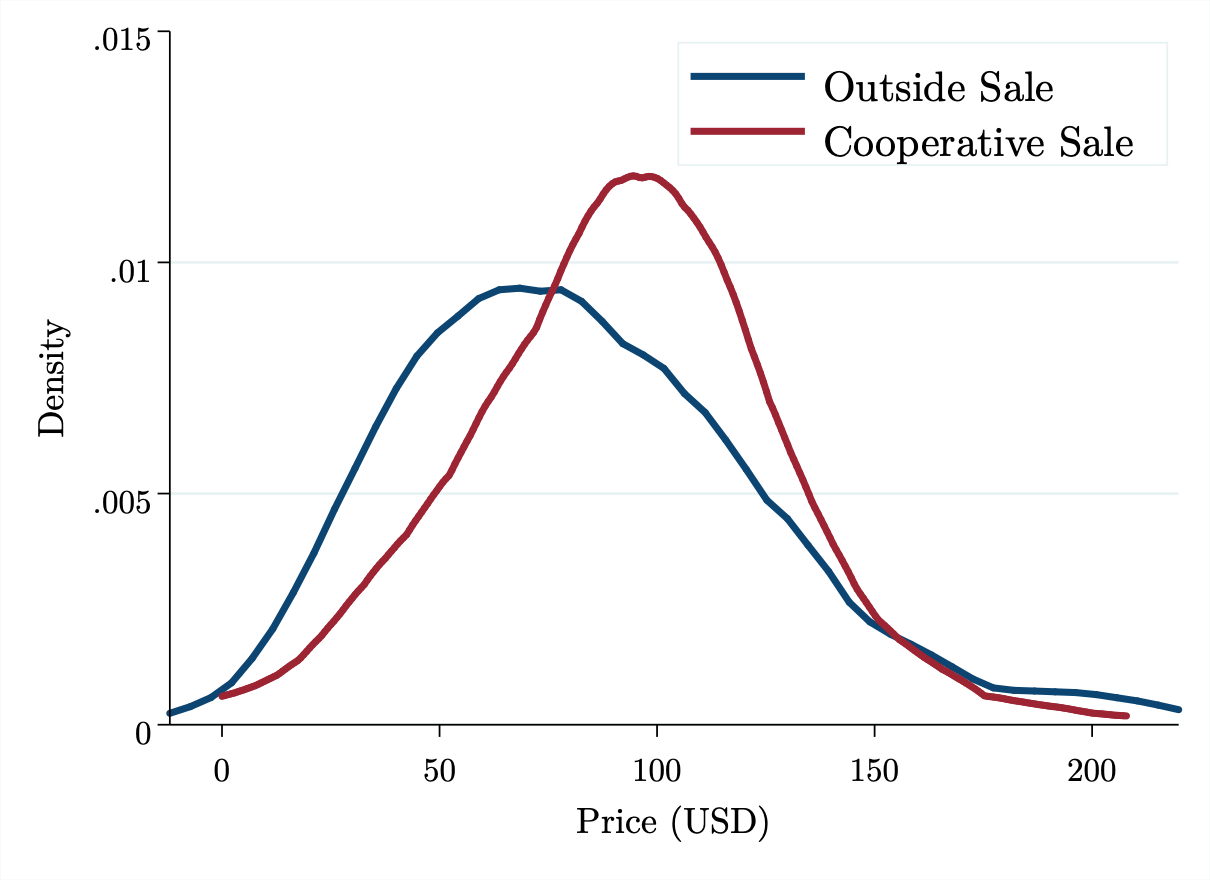
\includegraphics[width=\linewidth,trim=4 4 4 4,clip]{E2_PriceDensity_Festival.png} 
    \end{subfigure}
    \hfill
    \begin{subfigure}[t]{0.4\textwidth}
        \centering
        \caption{Non-Festival Season} \label{figure:E2_PD_NonFest}
        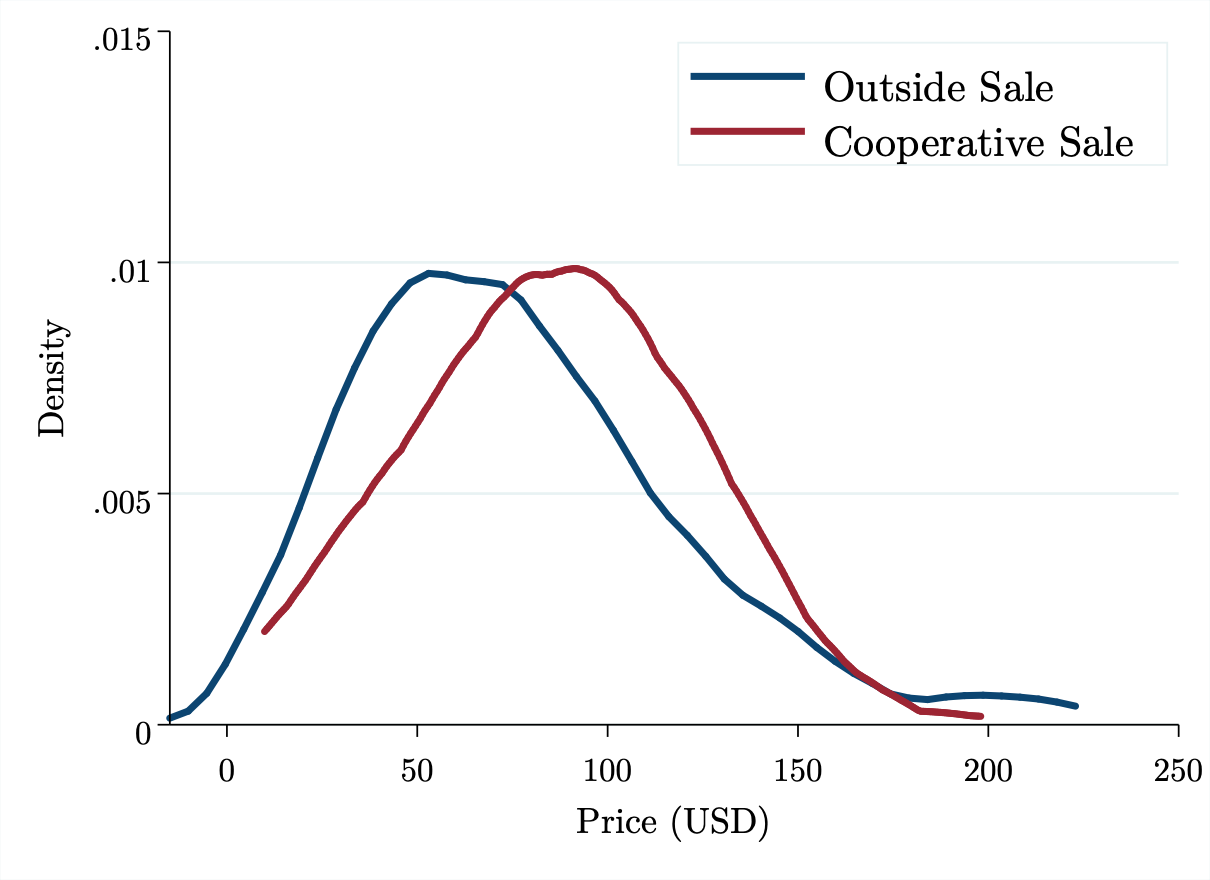
\includegraphics[width=\linewidth,trim=4 4 4 4,clip]{E2_PriceDensity_NonFest.png} 
    \end{subfigure}
\end{figure}

Table (\ref{table:E2_ss_reason}) reports the reasons that households provided for side-selling in the year prior to data collection. For each sale that was made outside of the cooperative in this time-period, households were asked to select the reason(s) that best explain their decision to side-sell. Fewer than ten percent report side-selling due to receiving delayed payments from the cooperative, less than 20\% report doing so because the cooperative's sale point was too far away and nearly 30\% stated that they side-sold because the cooperative did not arrange a sale at the time that they sold goats. Perhaps most important is that nearly half of side-selling households indicate that they sold outside of the cooperative because a local trader offered them a higher price. This further suggests that producers are opting not to sell through the cooperative when the price is not large-enough to sufficiently offset the added costs of group participation.

\singlespacing
\begin{table}[H]
  \centering
  \caption{Reasons for Side-Selling}
  \label{table:E2_ss_reason}
  \scalebox{.85}{
  \begin{tabularx}{.9\linewidth}{lcc}
\hline \noalign{\smallskip} & N & \% of households\\
\noalign{\smallskip}\hline \noalign{\smallskip}Delayed payment with cooperative & 1,070.00 & 8.13\\
Cooperative sale point is too far away & 1,070.00 & 18.41\\
Trader offered a higher price & 1,070.00 & 49.72\\
Cooperative did not arrange a sale at this time & 1,070.00 & 29.53\\
\hline
\multicolumn{3}{@{}p{.9\textwidth}}
{\footnotesize{\textit{Notes}: For each sale that was made outside of the cooperative in the year prior to data collection, households were asked to select the option(s) that best represented their decision to side-sell. The percentage of households column reports the percentage of households that selected each option at least once.}}
  \end{tabularx}}
\end{table}
\doublespacing

Table (\ref{table:E2_ss_perception}) displays the perception of side-selling among producers in my sample. In a hypothetical scenario in which the cooperative had 100 goats to sell, members believe that 67\% would be sold through the cooperative, approximately 25\% would be sold outside of the cooperative and less than 8\% would go unsold. As outlined in section (\ref{sec:background}), the total number of producers participating in a given sale can increase the bargaining position of the cooperative and increase the price received. With imperfect information, members may have to resort to educated guesses about the number of other members that will participate in a sale, and whether the cooperative will reach the threshold number that makes cooperative sales worthwhile \citep{aflagah_cheap_2019}. This data suggests that cooperative members in this setting believe that far more members are selling through the cooperative than actually do so. 

\singlespacing
\begin{table}[H]
  \centering
  \caption{Perception of Side-Selling}
  \label{table:E2_ss_perception}
  \scalebox{.85}{
  \begin{tabularx}{.9\linewidth}{lcc}
\hline \noalign{\smallskip} & N & \% of sales\\
\noalign{\smallskip}\hline \noalign{\smallskip}Sold through the cooperative \hspace{3cm} & 2,856.00 & 67.39 \\
Sold outside of the cooperative & 2,856.00 & 24.70 \\
Not sold at all & 2,856.00 & 7.89 \\
\hline
\multicolumn{3}{@{}p{.9\textwidth}}
{\footnotesize{\textit{Notes}: Each household was asked: in a hypothetical scenario in which the cooperative had 100 goats ready to be sold, how many do you believe would be sold through the cooperative, outside of the cooperative and not sold at all.}}
  \end{tabularx}}
\end{table}
\doublespacing

Finally, table (\ref{table:E2_ss_comp}) compares the characteristics of members that exclusively sell goats through the cooperative and those who exclusively side-sell. While there is no significant difference in age or distance to the cooperative between the two groups, exclusive cooperative sellers are more likely to be literate, have a larger number of goats, attended more self-help group meetings and were contacted about cooperative sales more frequently than outside sellers. Exclusive side-sellers had been members of their cooperative for longer and believed that a higher share of goats would be sold outside of the cooperative than those that exclusively sold through the cooperative. 

\singlespacing
\begin{table}[H]
  \centering
  \caption{Member Characteristics: Cooperative vs. Side-Selling}
  \label{table:E2_ss_comp}
  \scalebox{.7}{
  \begin{tabularx}{1.2\linewidth}{llll}
\hline \noalign{\smallskip} & Cooperative Sellers & Side-Sellers & Difference \\
\noalign{\smallskip}\hline \noalign{\smallskip} Age (years) & 39.97 & 40.24 & -0.27 \\
Literacy (0/1) & 0.84 & 0.76 & 0.08*** \\
Distance from cooperative (miles) & 1.29 & 1.19 & 0.10 \\
Pre-sales herd size (count) & 11.03 & 8.99 & 2.04*** \\
Cooperative Membership Length (months) & 33.89 & 39.21 & -5.32*** \\
SHG meetings attended in last 6-months (count) & 5.82 & 5.50 & 0.32***   \\
Share of goats perceived to be side-sold (percent) & 12.92 & 27.94 & -15.03*** \\
Times contacted about cooperative sales in last 6-months (count) & 1.89 & 0.81 & 1.09*** \\
\hline
\multicolumn{3}{@{}p{.9\textwidth}}
{\footnotesize{\textit{Notes}:}}
  \end{tabularx}}
\end{table}
\doublespacing


% --------------------------------------
\section{Empirical Strategy} \label{sec:E2_emp}

In this section, I outline my empirical strategy for estimating the impact of selling goats through a cooperative as opposed to side-selling. I will estimate the Average Treatment Effect on the Treated (ATT) for a series of outcome variables, following the approach outlined in Farrell (2015). This procedure combines “doubly robust” treatment effect estimation with model selection using the LASSO algorithm. I use the LASSO to select from a set of variables that are potentially correlated with the outcomes of interest as well as the selling decision (cooperative or side-selling). By relying on the LASSO for variable selection, I minimize ad hoc modeling assumptions and select variables in a way that results in valid inference under standard conditions.

\subsection{Identification}

Identifying the ATT requires two assumptions that jointly form what is referred to as strong ignorability \citep{rosenbaum and Ruben, 1983}. The first assumption states that the untreated potential outcome is mean independent of treatment status (i.e. the Conditional Independence Assumption (CIA)). This assumption can be expressed as follows

\begin{equation}
E\left[y_{i}^{0} \mid d_{i}, \mathbf{x}_{i}\right]=E\left[y_{i}^{0} \mid \mathbf{x}_{i}\right]
\end{equation}

Where $d_i = 1$ if producer $i$ sells through the cooperative and $d_i = 0$ if she side-sells, $y^{d}_{i}$ is the value of a potential outcome variable that would be observed if producer $i$ had selling status $d$ and $x_i$ is a vector of covariates. The second component of strong ignorability is an overlap condition on the propensity score:

\begin{equation}
p\left(d_{i}=1 \mid \mathbf{x}_{i}\right)<1 \text { for all } \mathbf{x}_{i} \in \mathbf{X}_{\mathbf{l}}
\end{equation}

where $\mathbf{X}_{\mathbf{l}}$ represents the set of all values of the vector of covariates observed among households participating in cooperative sales. This assumption ensures that there are valid control households for all treated households. When combined with the Stable Unit Treatment Value Assumption (SUTVA) --- that there are no program spillovers and all beneficiaries receive the same intervention --- the conditions given in (1) and (2) are sufficient to identify the ATT of cooperative sales.

The channels through which SUTVA might be violated by cooperative sales include ...


\subsection{Estimation}

The above identifying assumptions ensure that unbiased and consistent estimation of the ATT is possible using matching methods and inverse probability weighting (Imbens, 2004). One key issue in estimating causal effects in observational studies in the presence of a large number of potential covariates and little theoretical guidance on proper functional form. While theory and contextual knowledge shed light on which key variables should be included as covariates, it is often not clear whether a given variable should also be included as a polynomial or interaction term. This situation results in researchers informally choosing between numerous potential specifications, often with no clear indication of which is best. Perhaps most importantly, the resulting inference rarely accounts for this specification search and therefore is not robust to model selection mistakes (Danilov and Magnus, 2004; Farell, 2015). 

This has motivated a recent literature applying machine-learning (ML) algorithms to the estimation of average treatment effects (Belloni et al., 2014). While the LASSO is a variable selection algorithm that builds models with excellent predictive properties, it requires a valid identification strategy to estimate treatment effects with observational data (Belloni et al., 2014).

The LASSO algorithm constrains the sum of the absolute values of the regression coefficients to be less than a ``tuning parameter,'' thereby forcing some coefficients to zero. Perhaps most important for modern empirical research is that the LASSO can be used when the pool of covariates is larger than the sample size, an increasingly common feature among household-level datasets. As long as the true conditional mean function can be closely approximated by a model using fewer covariates than observations, the LASSO can serve as an accurate model selection algorithm. Constructing accurate confidence intervals for causal effects after performing model selection with the LASSO has been demonstrated to be relatively simply (Belloni et al., 2014; Farrell, 2015).

I estimate and perform hypothesis testing on the ATT of cooperative goat sales following the approach outlined in Farrell (2015). This method includes separate steps for model selection, estimation, and inference. In the model selection stage, the LASSO is applied to a logistic model of the propensity score using the entire sample, and then to a regression model (logit for binary outcomes, linear for continuous outcomes) for each outcome of interest using only the control group. For the propensity score and each outcome, I obtain LASSO results under 100 different values of the tuning parameter. By iterating through successively smaller values of the tuning parameter, I increase model complexity from one parameter (i.e. the intercept) to $N + 1$ parameters, where $N$ is the size of the estimation sample. The LASSO constraint ensures identification of the model with $N + 1$ parameters.

The covariates with non-zero coefficients under each value of the LASSO tuning parameter define alternative sets of covariates that could be used in ATT estimation. I compare the alternative sets of covariates using five-fold cross validation. The set of covariates that minimizes the sample average of a goodness of fit statistic generated through cross validation is used in ATT estimation. For the propensity score model, my goodness of fit measure is the deviance:

\begin{equation}
\frac{-2}{N} \sum_{i=1}^{N}\left[d_{i} \mathbf{x}_{i}^{\prime} \hat{\beta}-\ln \left(1+\exp \left(\mathbf{x}_{i}^{\prime} \hat{\beta}\right)\right)\right]
\end{equation}

For each observation $i$, the estimated parameter vector $\hat{\beta}$̂ is obtained using the cross validation blocks that do not include $i$.

The cross validation procedure for my outcome variables proceeds in a similar fashion. The major differences are that the sample is restricted to households that did not sell goats through their cooperative and the outcome models are estimated by OLS when the dependent variable is continuous. When evaluating linear models, my goodness of fit statistic is mean squared prediction error for non-participant households:

\begin{equation}
\frac{1}{\sum_{i=1}^{N}\left(1-d_{i}\right)} \sum_{i=1}^{N}\left(1-d_{i}\right)\left(y_{i}-\hat{y}_{i}\right)^{2}
\end{equation}

For each observation $i$, the fitted value $\hat{y}_{i}$̂ is generated from a model estimated using the four cross validation folds that do not include i. For binary outcomes, the goodness of fit statistic is the deviance given in equation ??, calculated using non-participants.

The pool of covariates entered into the LASSO algorithm includes the variables shown in Table 1 as well as several additional controls. ...

Once the final set of covariates is selected for the propensity score model as well as each outcome, the logit and regression models used to obtain the ATT are estimated without the LASSO constraint in order to avoid biasing model coefficients downwards. In other words, I use the “post-LASSO” estimator rather than the constrained estimator to construct my treatment effect estimator (Belloni et al., 2014; Farrell, 2015; Hastie, Tibshirani, and Wainwright, 2015). The estimated ATT for outcome $y$, $\widehat{ATT}$, is given by:

\begin{equation}
\begin{array}{l}
 \widehat{ATT} =\bar{y}_{1}-\frac{1}{N} \sum_{i=1}^{N}\left[\frac{d_{i} \hat{y}_{i}^{0}}{\hat{F}}+\frac{\left(1-d_{i}\right) \hat{\omega}_{i}\left(y_{i}-\hat{y}_{i}^{0}\right)}{\hat{p}}\right] \\
\hat{\omega}_{i}=\frac{\hat{p}\left(\mathbf{x}_{i}\right)}{1-\hat{p}\left(\mathbf{x}_{i}\right)}
\end{array}
\end{equation}

where $\bar{y}_1$ is the sample average of the outcome among cooperative sellers, $\hat{P}$ is the proportion of the sample participating in the treatment group, $\hat{p}\left(\mathbf{x}_{i}\right)$ is the estimated propensity score, and $\hat{y}_{i}^{0}$ is the value of the outcome in the absence of cooperative participation as predicted by OLS or the fitted probability as predicted by a logit regression, depending on whether the outcome is continuous or binary. As shown in the appendix, the ATT estimator in equation (5) is “doubly robust”. That is, the ATT estimator is unbiased when either the model for the outcome or that of the propensity score is correctly specified (Wooldridge, 2007). 


\subsection{Inference}

In the inference stage, I create t-statistics using the square root of the variance estimator \citet{farrell_robust_2015}:

\begin{equation}
\frac{1}{N}\left[\sum_{i=1}^{N} \frac{d_{i}\left(y_{i}-\hat{y}_{i}^{0}-A \hat{T} T\right)^{2}}{\hat{P}^{2}}+\frac{\left(1-d_{i}\right) \hat{\omega}_{i}\left(y_{i}-\hat{y}_{i}^{0}\right)^{2}}{\hat{P}(1-\hat{P})}\right]
\end{equation}

The ATT estimator is asymptotically normal and the variance esti- mator is robust to heteroscedasticity of unknown form. Farrell (2015) uses critical values from the standard normal distribution in hypothesis testing. In order to make inference appropriately conservative given my small sample, I use critical values from a t distribution with degrees of freedom equal to the total number of households in the data set minus the total number of parameters in the propensity score and outcome models.

I adjust inference for multiple hypothesis testing by ... 

% --------------------------------------
\section{Results}

\subsection{Matching and Covariate Balance}

\begin{figure}[H]
\caption{Linearized Propensity Score Distribution}
    \centering
    \begin{subfigure}[t]{.49\textwidth}
    \centering
        \caption{Full Sample} \label{figure:E2_PD_Annual}
        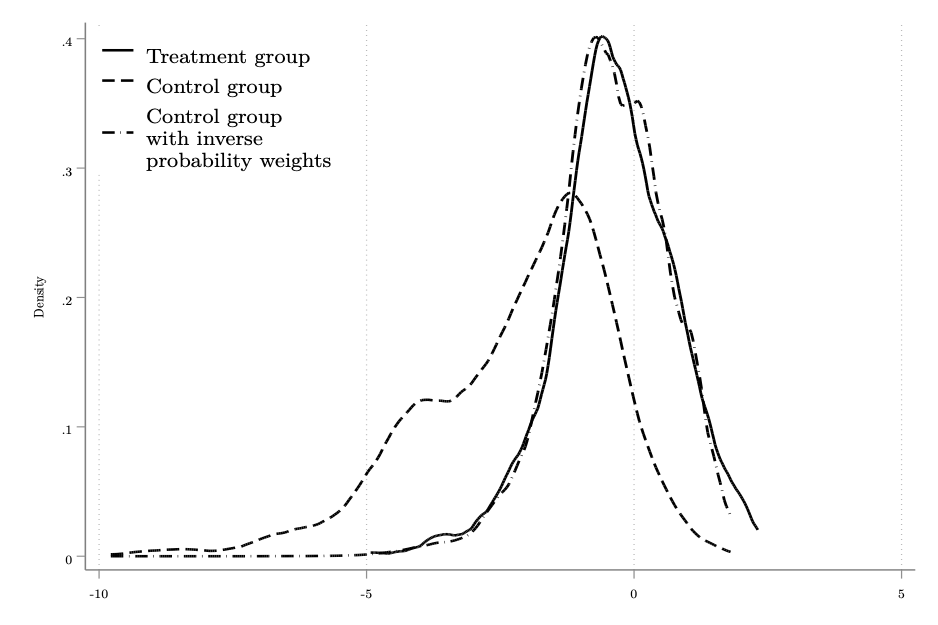
\includegraphics[width=\linewidth,trim=4 4 4 4,clip]{pscore_dens.png} 
    \end{subfigure}
    \begin{subfigure}[t]{0.49\textwidth}
        \centering
        \caption{Trimmed Sample} \label{figure:E2_PD_Festival}
        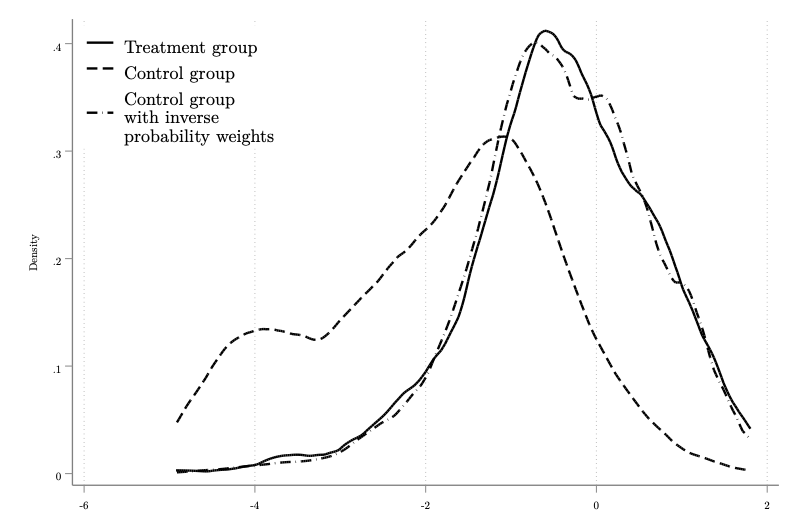
\includegraphics[width=\linewidth,trim=4 4 4 4,clip]{pscore_dens_comm.png} 
    \end{subfigure}
\end{figure}

\singlespacing
\begin{table}[H]
\caption{Covariate Balace}
\scalebox{.63}{
\begin{tabular}{llllllll}
\hline
 & \multicolumn{3}{l}{Unweighted sample} & & \multicolumn{3}{l}{Inverse probability weighted sample} \\ \cline{2-4} \cline{6-8}
 & Treatment Mean & Control Mean & p-value & & Treatment Mean & IPW control Mean & p-value   \\
 \hline
linearized pscore & -0.37 & -2.19 & 0.000 & & -0.37 & -0.43 & 0.528 \\
Altitude$^2$ & 7.2e+05 & 5.9e+05 & 0.004 & & 7.2e+05 & 7.3e+05 & 0.929 \\
Literacy & 0.85 & 0.76 & 0.000 & & 0.85 & 0.86 & 0.764 \\
Literacy X No. floors  & 0.53 & 0.44 & 0.001 & & 0.53 & 0.53 & 0.936 \\
Literacy$^2$ & 0.85 & 0.76 & 0.000 & & 0.85 & 0.86 & 0.764 \\
Age X Primary activity is agriculture & 29.37 & 28.45 & 0.425 & & 29.37 & 29.44 & 0.958 \\
Age X Dirt floors & 18.02 & 22.09 & 0.001 & & 18.02 & 17.71 & 0.830 \\
Age X No. cooperative services & 382.07 & 295.54 & 0.000 & & 382.07 & 381.64 & 0.965 \\
Household size X Altitude & 3572.99 & 3402.70 & 0.426 & & 3572.99 & 3422.48 & 0.612 \\
Household size X Primary activity is agriculture & 4.35 & 3.99 & 0.067 & & 4.35 & 4.36 & 0.960 \\
Household size X Leadership role & 0.76 & 0.50 & 0.005 & & 0.76 & 0.74 & 0.871 \\
Primary activity is agriculture X Altitude & 531.47 & 472.18 & 0.052 & & 531.47 & 528.92 & 0.960 \\
Primary activity is agriculture X Leadership role  & 0.10 & 0.07 & 0.122 & & 0.10 & 0.11 & 0.702 \\
Primary activity is agriculture X Goat empowerment index &  5.68 & 6.34 & 0.039 & & 5.68 & 5.99 & 0.433 \\
Primary activity is agriculture X No. cooperative services & 6.72 & 4.75 & 0.000 & & 6.72 & 6.85 & 0.689 \\
Leadership role X Altitude & 87.28 & 62.05 & 0.077 & & 87.28 & 96.47 & 0.786 \\
Leadership role X Dirt floors & 0.06 & 0.05 & 0.488 & & 0.06 & 0.05 & 0.927 \\
Leadership role X Distance from cooperative & 0.19 & 0.12 & 0.016 & & 0.19 & 0.17 & 0.756 \\
Leadership role X Goat empowerment index & 1.47 & 0.77 & 0.000 & & 1.47 & 1.47 & 0.996 \\
Leadership role X No. cooperative services & 1.51 & 0.71 & 0.000 & & 1.51 & 1.47 & 0.898 \\
Distance from cooperative X Altitude & 565.92 & 756.39 & 0.005 & & 565.92 & 556.19 & 0.842 \\
Goat empowerment index X Altitude & 4131.68 & 4873.96 & 0.019 & & 4131.68 & 4282.96 & 0.762 \\
Goat empowerment index X Dirt floors & 3.51 & 4.90 & 0.000 & & 3.51 & 3.40 & 0.758 \\
Goat empowerment index X Distance from cooperative & 8.08 & 11.45 & 0.000 & & 8.08 & 8.38 & 0.640 \\
Goat empowerment index X No. floors & 4.42 & 4.83 & 0.189 & & 4.42 & 4.56 & 0.730 \\
Membership length X Altitude & 1674.00 & 1848.54 & 0.138 & & 1674.00 & 1701.38 & 0.864 \\
Membership length X Leadership role & 0.31 & 0.19 & 0.022 & & 0.31 & 0.31 & 0.980 \\
Membership length X Dirt floor & 1.27 & 1.62 & 0.002 & & 1.27 & 1.28 & 0.950 \\
Membership length$^2$ & 9.06 & 12.77 & 0.000 & & 9.06 & 9.29 & 0.685 \\
No. cooperative services & 9.65 & 7.45 & 0.000 & & 9.65 & 9.66 & 0.952 \\
No. cooperative services X Altitude & 5725.06 & 3861.08 & 0.000 & & 5725.06 & 5710.08 & 0.977 \\
No. cooperative services X Goat empowerment index & 78.80 & 64.49 & 0.000 & & 78.80 & 79.13 & 0.937 \\
No. cooperative services$^2$ & 100.23 & 71.21 & 0.000 & & 100.23 & 100.53 & 0.928 \\
No. floors X Dirt floors & 0.28 & 0.34 & 0.020 & & 0.28 & 0.27 & 0.806 \\
No. floors X Distance from cooperative & 0.69 & 0.61 & 0.184 & & 0.69 & 0.74 & 0.586 \\
Herd size X No. SHG meetings & 70.75 & 57.38 & 0.000 & & 70.75 & 67.91 & 0.458 \\
Herd size X Primary activity is agriculture & 8.67 & 7.35 & 0.017 & & 8.67 & 8.56 & 0.861 \\
Herd size X Leadership role & 2.23 & 1.39 & 0.034 & & 2.23 & 2.04 & 0.701 \\
Herd size X Distance from cooperative & 15.14 & 14.49 & 0.636 & & 15.14 & 16.71 & 0.568 \\
Herd size X Goat empowerment index & 95.48 & 84.45 & 0.038 & & 95.48 & 93.79 & 0.818 \\
Herd size$^2$ & 217.23 & 215.45 & 0.960 & & 217.23 & 209.79 & 0.755 \\ \\
Observations & 427 & 1318 & & & 427 & 1318  &  \\
\hline
\multicolumn{8}{@{}p{1.6\textwidth}}
{\textit{Notes}: Propensity score estimated via a logit regression, with covariates selected using the logit LASSO. The LASSO tuning parameter was selected by five-fold cross validation as applied to the post-LASSO (i.e. unpenalized) model. The normalized differences show the difference in means divided by the pooled sample standard deviation as described in the text.}
\end{tabular}}
\end{table}
\doublespacing


\subsection{Average Treatment Effects on the Treated}

\singlespacing
\begin{table}[H]
\caption{Average Treatment Effects on the Treated}
\scalebox{.85}{
\begin{tabular}{lllllll}
\hline
Outcome & ATT & Percent impact & Standard error & p-value & q-value & 95\% Confidence Interval \\
\hline
Price (USD) & 14.83 & 18.43\% & 1.49 & 0.000 &  & (11.90, 17.76) \\ 
Goats sold (count) & 0.06 & 3.83\% & 0.05 & 0.222 & & (-0.04,  0.15) \\ 
Net goat income (USD) & 36.88 & 23.02\% & 7.57 & 0.000 & & (22.04, 51.71) \\ \\
Observations & 3004 &  &  &  &  & \\
\hline
\multicolumn{7}{@{}p{1\textwidth}}
{\textit{Notes}: }
\end{tabular}}
\end{table}
\doublespacing


\subsection{Heterogeneous Treatment Effects}

\subsection{Robustness Checks}



% --------------------------------------
\section{Discussion}

% --------------------------------------
\section{Conclusion}

%------------------------------------------%
\newpage
\bibliography {references}
%------------------------------------------%

\end{document}
